\documentclass{article}

\usepackage[utf8]{inputenc}
\usepackage{fullpage,amsmath,amssymb}
\usepackage{graphicx,caption, float}
\usepackage{fancyvrb,placeins,lscape, arydshln}
\usepackage[title]{appendix}
\usepackage{newtxtext,newtxmath, url}
\RecustomVerbatimCommand{\VerbatimInput}{VerbatimInput}{fontsize=\scriptsize}

\title{\textit{Get Pumped:} Water Points in Tanzania}
\author{Ethan Buck, Leyli Garryyeva, Gergana Gospodinova, and Xin Zhang}
\date{\today}

\begin{document}

\maketitle

\section{Problem Description}
This project stems from finding a data set from a competition on DrivenData.  The competition is called ``Pump it Up: Data Mining the Water Table'', and provides a data set with different water points.  There are six different types of water points:

\begin{enumerate}
    \item Cattle Trough
    \item Communal Standpipe
    \item Dam
    \item Hand Pump
    \item Improved Spring
    \item Other
\end{enumerate}

The goal is to accurately predict the operating condition of these water points located in Tanzania.  There are three different classes for this response variable, which are

\begin{enumerate}
    \item functional
    \item functional needs repair
    \item non functional
\end{enumerate}

Thus, this is a classification problem.  There are 39 different predictors for this data set, nine of which are continuous covariates.  Early data exploration reveals that none of these continuous covariates appear to resemble a normal distribution, and thus LDA and QDA most likely are not suitable choices.  However, an adapted logistic regression may prove to be fruitful in this analysis, as well as a potential random forest model.  KNN classification may be suitable as well, since there are a large number of training observations (59,400).

Section \ref{dataClean} will discuss the data cleaning process.  Exploratory plots are shown in Section \ref{explore}.  The KNN analysis follows in Section \ref{knn}.  Section \ref{logistic} goes through the logistic regression results, and Section \ref{randForest} explains the results from random forests.

\section{Data Cleaning} \label{dataClean}
The data cleaning process was mostly straightforward, though there were some key discoveries that helped immensely for the model fitting.

We first started by getting rid of factors that had too many levels, as we feared adding hundreds of parameters was unnecessary and would lead to over-fitting by the model.  After inspecting the data to see how many levels there were for all of the factors, we set the boundary to be at most 21 levels for each factor.  The variables that were removed from this process were:

\begin{enumerate}
    \item date recorded: the date the row was entered. 356 levels
    \item funder: who funded the well. 1,898 levels
    \item installer: organization that installed the well. 2,146 levels
    \item wpt name: name of the water point if there is one. 37,400 levels
    \item subvillage: geographic location (also represented by other variables). 19,288 levels
    \item lga: geographic location (also represented by other variables). 125 levels
    \item ward: geographic location (also represented by other variables). 2092 levels
    \item scheme name: who operates the water point. 2697 levels
\end{enumerate}

These variables also make sense to remove, as they appear to be more miscellaneous information that would not provide useful information for predictions (except for geographic location, which is represented by other variables remaining in the data set).  Additionally, the ``recorded by'' variable was a factor with only one level, which was ``GeoData Consultants Ltd'', and thus this was removed as well.

There are many categorical predictors, and after looking again at the structure of the dataset we realize that many of them are duplicates of others.  By this we mean that some columns are exactly the same, or that some predictors just group some of the labels together, but represent the same measurement.  We examined each variable using the table() R command, to see all of the unique label names and counts and compare them with their similar counterparts.  In most cases, we chose to keep the predictor with less labels (or the one that grouped together more categories) so that there will be less parameter estimates, saving important degrees of freedom.  However, if we thought that the labels should not have been grouped together, and that their responses would vary significantly, we chose to keep the predictor with more variables.  The choices are summarized in Table \ref{tab:repeatFactors}.

\begin{table}[h]
\center
\caption{Repeat factors that were removed due to containing the same type of information as others.}
\begin{tabular}{|c|c|}
\hline
     Removed predictors & Represented By \\
     \hline
     
extraction type, extraction type group   &  extraction type class \\
management  & management group \\
payment type    & payment   \\
water quality   & quality group   \\
quantity group     & quantity    \\
source type, source class  & source \\
waterpoint type   & waterpoint type group \\
\hline
\end{tabular}
\label{tab:repeatFactors}
\end{table}

There were minor relabeling of factor labels and grouping of certain labels together that did not have many counts into an ``other'' category, but these were the main steps taken in the data cleaning process.


\section{Exploratory Analysis} \label{explore}
We wanted to first see if LDA and QDA were potential models by checking for normal covariates.  We saw that there were a large number of factors in the data, and so we tried only considering the numerical predictors, and used histograms to see if we could rule out normal distributions.  These are shown in Figure \ref{fig:NonNormalHists}.  It is clear that all of these are far from being able to be assumed to follow normal distributions, and thus we presume that LDA and QDA models are not appropriate and would not yield predictive models.

\begin{figure}[h]
    \centering
    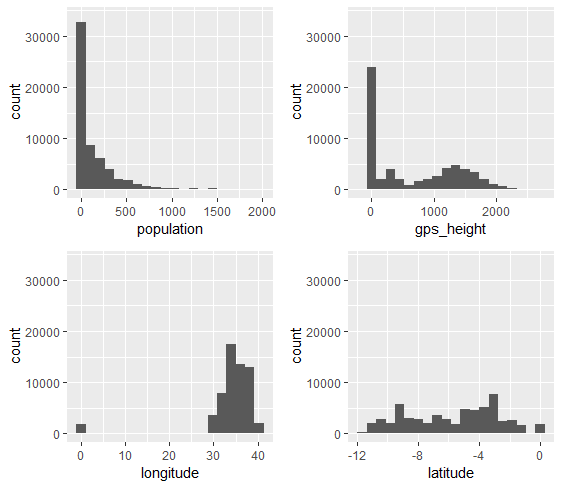
\includegraphics[width=0.6\textwidth]{Figures/HistsNotNormal.png}
    \caption{Histograms of some of the numerical predictors.}
    \label{fig:NonNormalHists}
\end{figure}

\section{KNN Classification} \label{knn}


\large
\section{Logistic Regression} \label{logistic}
This section describes attempt to predict the condition status of the water pump by means of multinomial logistic regression (MLR). The model was fit using \texttt{multinom} function from the \texttt{nnet} package in R to perform MLR. The package uses feed-forward neural networks with a single hidden-layer and \texttt{multinom} function fits multinomial log-linear models. MLR is an extension of a simple logistic regression that allows for predicting variables with three or more categories. 

The target categorical variables are \textsc{functional, functional needs repair,} and \textsc{non functional} which correspond to the status of the water pump's condition. Prior to fitting the model, the data was split in the ratio of $1/3$ and $2/3$ to create training and test datasets, respectively. 

The initial model included all the features and the accuracy rate for training data and testing data were 73.41$\%$ and 72.68$\%$, respectively. When applied to the whole training, the accuracy rate was 73.22$\%$. After submitting the predictions to the competition website we got the score of 71.43$\%$. Below is the confusion matrix associated with this model:

\begin{figure}[h]
    \centering
    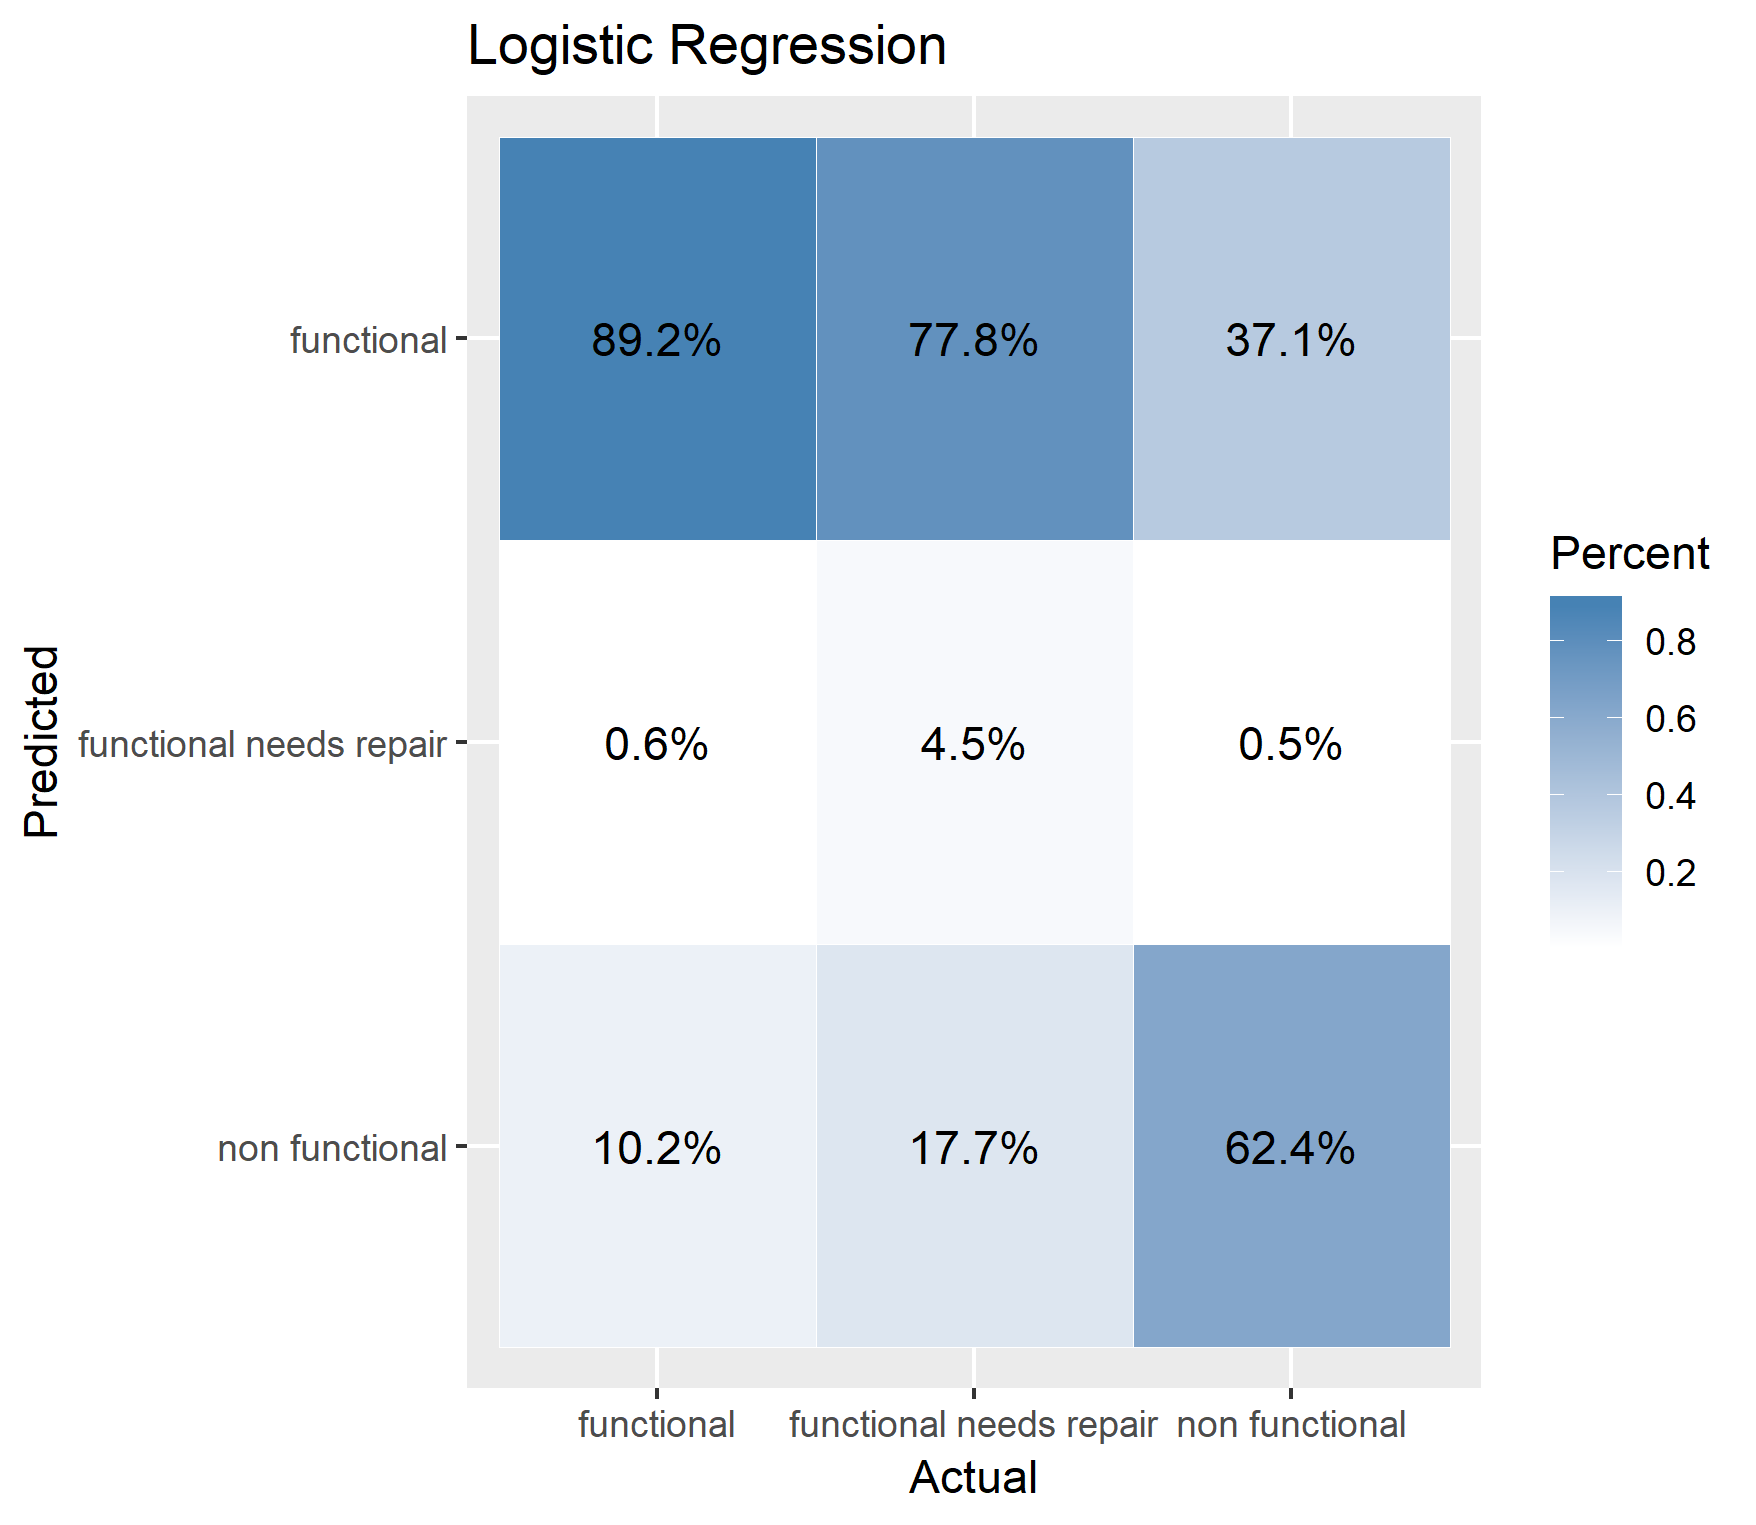
\includegraphics[width=0.6\textwidth]{LogConfMatrix.png}
    \caption{Confusion matrix for the logistic regression model.}
    \label{fig:NonNormalHists}
\end{figure}

The confusion matrix indicates that most of the inaccuracy is associated with miss-classification of the \textsc{functional needs repair} category with 95.5$\%$ overall error rate where 77.8$\%$ of this class is miss-classified as \textsc{functional} and 17.7$\%$ as \textsc{non functional}. The \textsc{non functional} category is the second most inaccurately classified category with 37.6$\%$ error rate where 37.1$\%$ of this class is miss-classified as \textsc{functional}. Lastly, only 10.8$\%$ of functional pumps were miss-classified. 

Further, the prediction accuracy was compared among several models with varying features and interactions between certain features, which seemed to perform better on the training data. The best rate recorded for the training data was equal to 73.68$\%$. However, after comparing the accuracy rates for the test data, it was found that the prediction accuracy did not differ between these models. The highest submission score achieved after all these attempts indicated 72.11$\%$ accuracy.  


\section{Random Forest Model} \label{randForest}


\section{Comparing the Models}
Figure \ref{fig:modelComp} shows a bar graph comparing the performances of the different models.  The models seem to perform very similarly on the functional water points, as there are so many observations of this type.  The models appeared to suffer much more when trying to predict the ``functional needs repair'' class, as there are not many observations in this  category (comparatively).  However, the oversampling method with the random forest model did help to combat this. This method also comes close to doing the best on the non functional class, and these two classes are the most important to predict correctly, as the purpose is to identify broken water points.

\begin{figure}[!h]
    \centering
    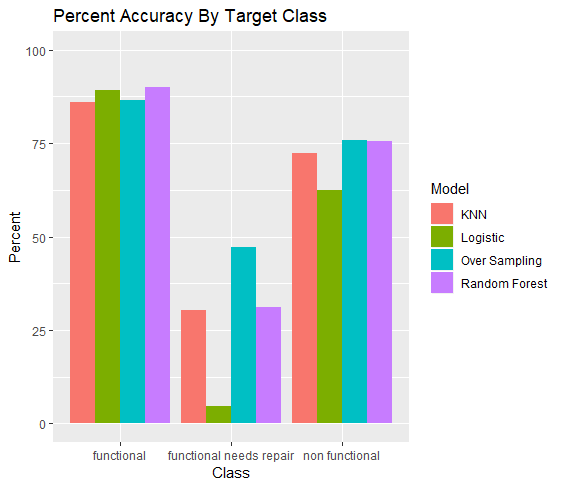
\includegraphics[width = 0.7\textwidth]{Figures/percentAccuracyByClass.png}
    \caption{Comparing the models' accuracy of predicting each target class}
    \label{fig:modelComp}
\end{figure}

Overall, the random forest model outperformed the other fitting methods, and this was without requiring excessive tuning of the model.  The pre-processing of the data was enough to be able to fit a relatively accurate model, and with the addition of oversampling, we were able to achieve more balanced class accuracy rates.

\newpage
\section{Appendix}



%The data set can be found online at \\ %\url{https://www.drivendata.org/competitions/7/pump-it-up-data-mining-the-water-table/page/23/}

\end{document}